\section{Evaluation}
\label{sec:eva}

The evaluation of our approach consists of two parts. In the first, we
evalute the benefit of using the dynamic programming query
optimization algorithm for Linked Data query processing in a
single-objective scenario. In the second part, we focus on the
multi-objective optimization approach proposed in this paper.

% \subsection{Single-objective Optimization with Dynamic Programming}

% \subsubsection{Systems}


% \subsubsection{Results}



% \begin{figure}[htb]
%   \centering
%   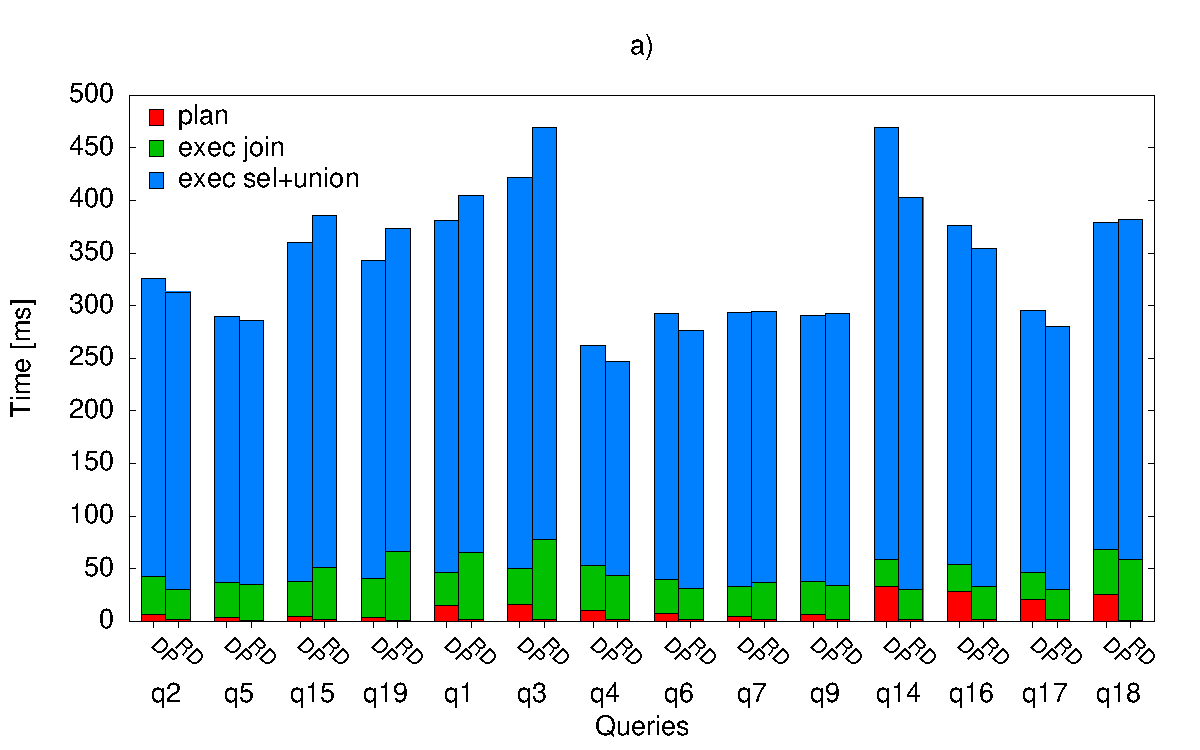
\includegraphics[width=\linewidth]{figs/exec_queries.pdf}
%   \caption{Results for execution}
%   \label{fig:exec_queries}
% \end{figure}


\begin{figure*}[htb]
  \centering
  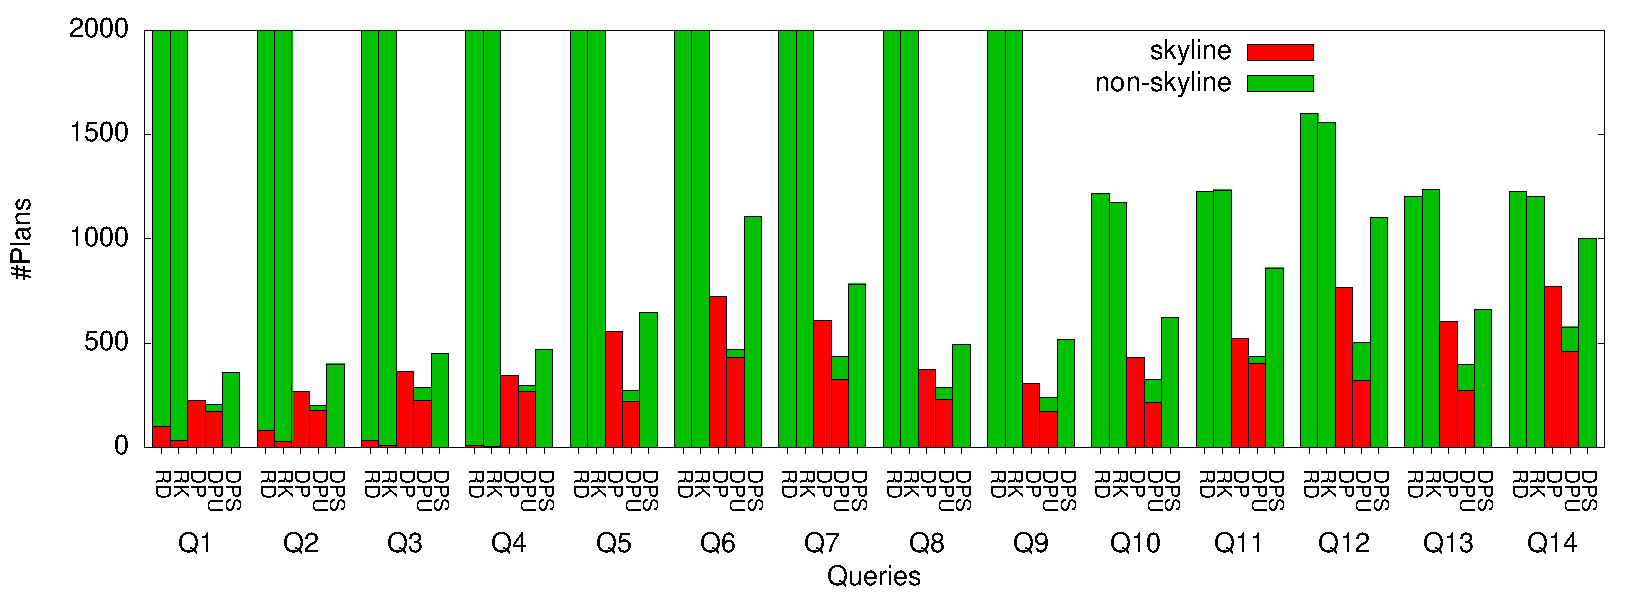
\includegraphics[width=0.7\linewidth]{figs/all_queries.pdf}
  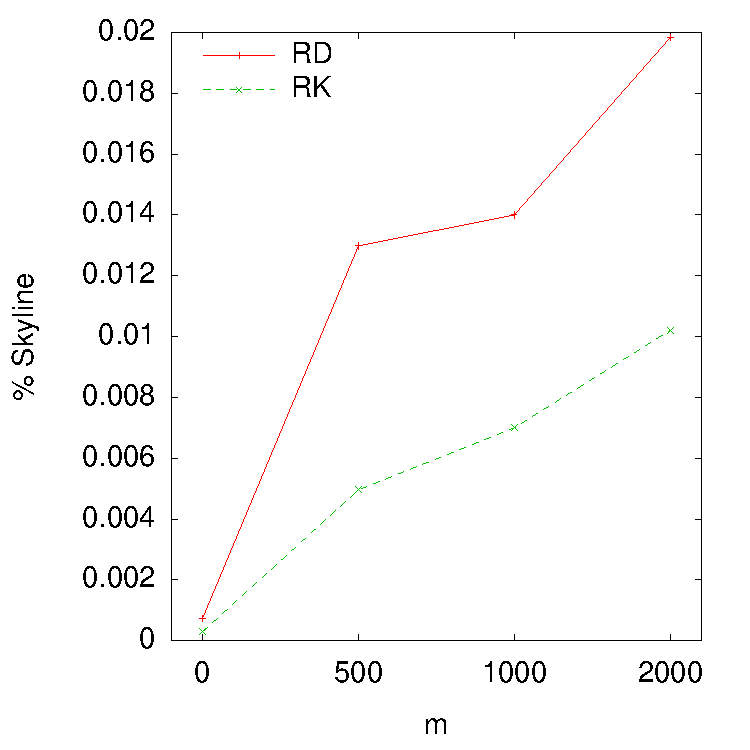
\includegraphics[width=0.29\linewidth]{figs/plans_skyline_by_m.pdf}
  \caption{a) Number of skyline and non-skyline plans for all queries
    and systems ($b=0.8, m=2000$), b) Skyline fraction for RD, RK for
    different value of $m$ ($b=0.8$).}
  \label{fig:queries}
\end{figure*}

%\subsection{Multi-objective Optimization with Dynamic Programming}

In the second part of the evaluation we examine the approach for
multi-objective optimization of Linked Data queries that was presented
in this paper. We will examine whether the dynamic programming
approach is effective and compare it with two baselines to assess the
quality of the generated plans.

\subsection{Systems}

\textbf{Baselines.} The Pareto-set of query plans that is generated by
our approach represents the trade-off between cost and cardinality and
allows the user to choose a plan according to her preferences. There
currently is no comparable baseline approach that also produces a
range of queries plans instead of a single one. We therefore created
two straightforward baselines, one based on random source selection
and one that first ranks sources by their relevance (this reflects
previous work on Linked Data query processing
\cite{harth_data_2010,ladwig_linked_2010}).

Both baselines first retrieve all relevant sources $D$ for a query $Q$
from the source index, i.e., $D = \bigcup_{q_i \in Q} I(q_i)$. As we
intend to create a whole range of query plans, both baselines now
create a set $\mathcal{D}$ of subsets of $D$ with sizes $\{1\ldots
|D|\}$ and $|\mathcal{D}| = |D|$. The baselines differ in how the
subsets are selected:
\begin{itemize}
\item Baseline RD randomly selects the $|D|$ subsets.
\item Baseline RK first ranks sources in $D$ by the number of
  contained triples that match query triple patterns, calculated as
  $score(d) = \sum_{t \in q} card_t(d)$. The subsets are then created
  by starting with the highest ranked source and then successively
  adding sources in order of their rank to obtain $|D|$ subsets in
  total.
\end{itemize}
Each element in $\mathcal{D}$ is a subset of all relevant source and
represents a combination of sources. For each of the source
combinations, we create a single query plan using a standard dynamic
programming optimizer (i.e., no multi-objective optimization). Sharing
of source scan operators is also employed where possible.

In all of the plans that were created in this fashion, any source that
contains data matching multiple triple patterns is always used as
input for all triple patterns, which is not the case for our
approach. In order to mimic this and thereby broaden the space of
possible plans, we create an additional set of $m$ plans for each
previously created plan by randomly removing inputs from the unions at
the root of access plans. In particular, to create a new plan from an
existing plan, for each union that is root of an access plan, we
remove a random subset of its input (selection) operators. If the
source scan operator that is input for a removed selection operator is
not shared it is also remove from the plan.

Any invalid plans that are constructed in this way (e.g., all inputs
of an union might have been) are discarded. In the end, each baseline
has at most of $m \cdot |D|$ plans.

\textbf{Our Approach.} We implemented two versions of our
approach. The first version (DP) obtains the complete set of
Pareto-optimal plans as described in the previous sections. The second
version (DPU) does not use bounds as described in
Section~\ref{sec:sharing} (i.e., while operator sharing is employed,
its effects are not taken into account during pruning) and therefore
will not compute the correct Pareto-optimal set of plans. However,
pruning is more effective and should lead to faster performance.

\textbf{Parameters.} Parameter $b$ specifies the benefit that is
assumed during query planning for sharing of source scan
operators. For example, with $b=0.8$ the planners assume that 80\% of
the source scan cost is saved, i.e., second and subsequent reads of a
source scan operator cost only 20\% of the first read.

For RD and RK, parameter $m$ describes the number of additional plans
that were generated by randomly remove selection and source scan
operators.

\subsection{Datasets and Queries}

We created 14 BGP queries of different sizes w.r.t. to the number of
triple patterns. We executed all queries using a link traversal
approach and recorded all retrieved sources. This dataset was then
indexed in a source index and used for the evaluation. The dataset
consists of 1,909,109 triples and contains data from various popular
open datasets, such as DBpedia, Freebase, New York Times, GeoNames,
LinkedMDB and others. Table~\ref{tab:queries} shows various
statistics for all evaluation queries.

As the source index contained too many sources for the multi-objective
optimization approach to deal with, we randomly aggregated sources
during the creation of access plans into a set of $k=5$ virtual
sources. The size of the virtual sources follows a Zipf distribution.

\begin{table}[htb]
  \centering
  \begin{tabular}{l|c|c|r}
    Query & \#Pat. & Shared [kT] & \#Res. \\%& Join-Sel. SD \\ 
    \hline

    Q2  & 3 & 1,393 & 24  \\%& 3.26\textsc{e}-5 \\
    Q5  & 3 & 1,425 & 13  \\%& 4.95\textsc{e}-5 \\
    Q15 & 3 & 1,401 & 11  \\%& 2.59\textsc{e}-5 \\
    Q19 & 3 & 1,434 & 836 \\%& 4.36\textsc{e}-5 \\
    \hline
    Q1  & 4 & 1,426 & 2   \\%& 1.30\textsc{e}-3 \\
    Q3  & 4 & 1,892 & 3   \\%& 1.89\textsc{e}-5 \\
    Q4  & 4 & 1,415 & 60  \\%& 9.58\textsc{e}-3 \\
    Q6  & 4 & 2,081 & 6   \\%& 2.62\textsc{e}-3 \\
    Q7  & 4 & 1,369 & 106 \\%& 2.75\textsc{e}-3 \\
    \hline
    Q9  & 5 & 1,405 & 17  \\%& 5.26\textsc{e}-3 \\
    Q14 & 5 & 1,830 & 20  \\%& 3.71\textsc{e}-3 \\
    Q16 & 5 & 2,396 & 1   \\%& 2.10\textsc{e}-3 \\
    Q17 & 5 & 1,409 & 1   \\%& 8.92\textsc{e}-3 \\
    Q18 & 5 & 1,007 & 2   \\%& 1.21\textsc{e}-4 \\
  \end{tabular}
  \caption{Query statistics: query name, number of patterns, number of
    triples (in thousands) contained in shared sources, number of results.}
  \label{tab:queries}
\end{table}

% \begin{table*}[htb]
%   \centering
%   \begin{tabular}{l|r|r|r|r|r|r|r|r|r|r|r|r|r|r|r|r}
%  & RD & RK & DP & DPU & RD & RK & DP & DPU & RD & RK & DP & DPU & RD & RK & DP & DPU \\
%     \hline               
                                                                                                               
%  & \multicolumn{4}{c}{Q2} & \multicolumn{4}{|c|}{Q5} & \multicolumn{4}{c}{Q15} & \multicolumn{4}{|c}{Q19}  \\

%     \hline                                                                                                   

%     \#Plans   & 1702 & 1853 & 673   & 619  & 1382 & 1871 & 446   & 446   & 2376 & 3263 & 634   & 634   & 3817 & 3240 & 761   & 761   \\
%     \#Skyline & 153  & 155  & 673   & 575  & 106  & 176  & 446   & 446   & 13   & 40   & 634   & 634   & 41   & 46   & 761   & 761   \\ 
%     \%Skyline & 22.7 & 23.0 & 100.0 & 85.4 & 23.8 & 39.5 & 100.0 & 100.0 & 2.1  & 6.3  & 100.0 & 100.0 & 5.4  & 6.0  & 100.0 & 100.0 \\
%     Time [s]  & 1.06 & 0.92 & 1.14  & 0.62 & 0.78 & 1.03 & 0.75  & 0.53  & 1.05 & 1.14 & 1.21  & 0.64  & 1.07 & 1.05 & 1.58  & 0.77  \\
  
%     \hline
%     \hline

%  & \multicolumn{4}{c}{Q1} & \multicolumn{4}{|c|}{Q3} & \multicolumn{4}{c|}{Q4} & \multicolumn{4}{c}{Q6} \\

%     \hline

%     \#Plans   & 3945 & 5362 & 866   & 832  & 4571 & 5153 & 901   & 847  & 1471 & 1306 & 453   & 465  & 954  & 1340 & 354   & 318  \\
%     \#Skyline & 0    & 0    & 866   & 689  & 0    & 0    & 901   & 699  & 1    & 0    & 453   & 434  & 0    & 1    & 354   & 283  \\ 
%     \%Skyline & 0.0  & 0.0  & 100.0 & 79.6 & 0.0  & 0.0  & 100.0 & 77.6 & 0.2  & 0.0  & 100.0 & 95.8 & 0.0  & 0.2  & 100.0 & 79.9 \\
%     Time [s]  & 1.53 & 1.67 & 7.64  & 1.60 & 1.53 & 1.62 & 10.05 & 1.80 & 1.61 & 1.29 & 1.37  & 0.75 & 1.14 & 1.33 & 1.35  & 0.70 \\

%     \hline
%     \hline

%  & \multicolumn{4}{c}{Q7} & \multicolumn{4}{|c|}{Q9} & \multicolumn{4}{c|}{Q14} & \multicolumn{4}{c}{Q16} \\

%     \hline

%     \#Plans   & 2566 & 3913 & 1035  & 813  & 2622 & 3450 & 689   & 655  & 429  & 436  & 284   & 281  & 1485 & 2265 & 685   & 663  \\
%     \#Skyline & 1    & 0    & 1035  & 781  & 0    & 0    & 689   & 637  & 0    & 0    & 284   & 281  & 0    & 0    & 685   & 583  \\ 
%     \%Skyline & 0.1  & 0.0  & 100.0 & 75.5 & 0.0  & 0.0  & 100.0 & 92.5 & 0.0  & 0.0  & 100.0 & 98.9 & 0.0  & 0.0  & 100.0 & 85.1 \\
%     Time [s]  & 1.91 & 1.50 & 20.88 & 2.28 & 1.80 & 1.64 & 23.64 & 2.56 & 1.33 & 1.21 & 0.91  & 0.41 & 1.82 & 1.99 & 14.31 & 2.38 \\

%     \hline
%     \hline

%  & \multicolumn{4}{c}{Q17} & \multicolumn{4}{|c|}{Q18} & \multicolumn{8}{c}{} \\

%     \hline

%     \#Plans   & 837  & 1022 & 398   & 286   & 1021 & 1192 & 633   & 633   & \multicolumn{8}{c}{} \\
%     \#Skyline & 1    & 0    & 398   & 286   & 0    & 0    & 633   & 633   & \multicolumn{8}{c}{} \\ 
%     \%Skyline & 0.2  & 0.0  & 100.0 & 100.0 & 0.0  & 0.0  & 100.0 & 100.0 & \multicolumn{8}{c}{} \\
%     Time [ms] & 1.67 & 1.70 & 2.68  & 0.66  & 1.53 & 1.58 & 4.15  & 1.35  & \multicolumn{8}{c}{} \\

%   \end{tabular}
%   \caption{Results for all queries, with $m=2000$ and $b=0.8$ for RD and RK.}
%   \label{tab:res}
% \end{table*}

\subsection{Setting}
All systems were implemented in Java. The query planner is
single-threaded, whereas the execution engine uses multiple
threads. All experiments were executed on a 2009 Macbook Pro with a
2.4 GHz Intel Core 2 Duo processor, 4GB RAM (of which 1GB was assigned
to the Java VM) and a Crucial m4 128GB solid-state disk.


\subsection{Results}

\textbf{Overall.} Fig.~\ref{fig:queries}a shows an overview over all
evaluation queries and displays the number of plans that were
generated by each system, split into skyline and non-skyline (i.e.,
dominated) plans. The number of skyline plans was determined by
collecting all plans of a particular query for all systems in one set
and then pruning all dominated plans. 

We can see that DP produces only skyline plans and that there are many
DPU plans that are part of the skyline (56\% on average). However, the
RD and RD baselines generate almost no skyline plans (3\% and 1\% on
average). 

Fig.~\ref{fig:queries}b shows the skyline fraction (i.e., the fraction
of the DP skyline) found by RD and RK for different values of $m$. We
see that for larger values of $m$ the skyline fraction is higher,
i.e., the larger plan space created by randomly removing union inputs
is necessary to find skyline plans.

\textbf{Effect of Query Size.} Figs.~\ref{fig:pareto_tp}a+b show the
planning time and found skyline fraction for different query sizes
(i.e., number of triple patterns). An increased number of triple
patterns results in a larger search space for the query optimizer: for
all systems planning time increases with the number of triple
patterns. However, the DP algorithm is much more affected than DPU, RK
and RD. Going from 3 to 5 triple patterns, the planning time of DP
increases by a factor of 87.7 while the planning time for DPU only
increases by a factor of 16, and RD and RK are largely unaffected. The
high increase in planning time for 5 triple patterns is largely due to
query Q16. Without Q16, the factors decrease to 54.9 and 10.5 for DP
and DPU, respectively.

Fig.~\ref{fig:pareto_tp}b shows the fractions of the complete plan
skyline (i.e., the plans computed by DP) that the systems are able to
calculate for different query sizes. Whereas for 3 triple patterns the
baselines RD and RK are able to find 17\% and 6\% of the skyline, no
skyline plans are found for 4 and 5 triple patterns. DPU also performs
better for 3 triple patterns, where 70\% of the skyline is found (54\%
for 4 and 5 triple patterns). For more triple patterns the space of
possible plans is much larger, which is why especially the baselines
perform much worse.

\begin{figure}[htb]
  \centering
  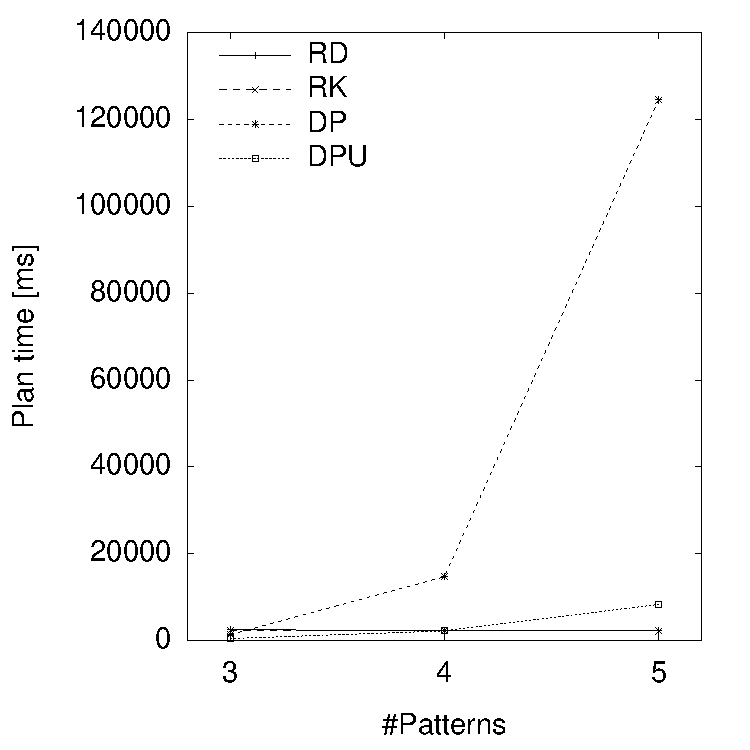
\includegraphics[width=0.49\linewidth]{figs/pareto_plan_tp.pdf}
  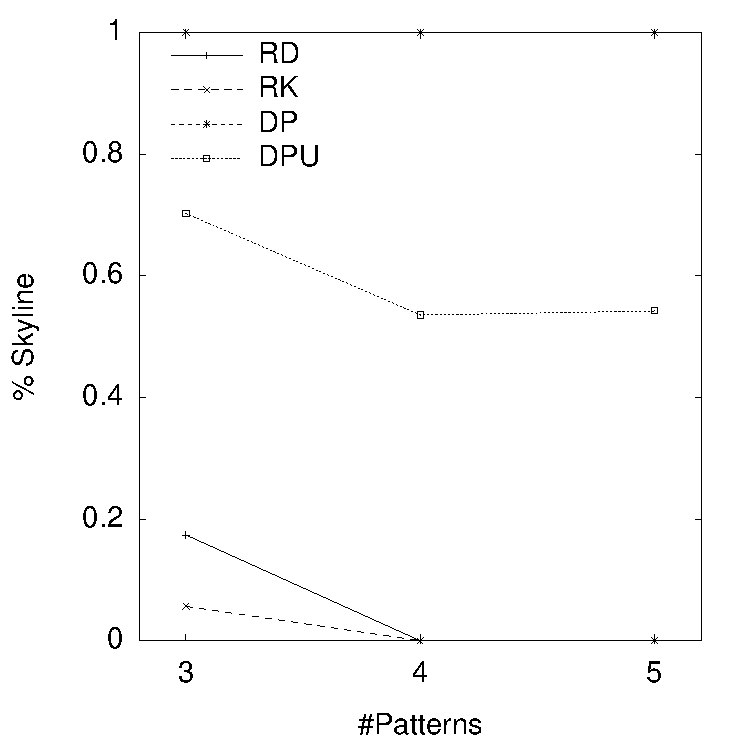
\includegraphics[width=0.49\linewidth]{figs/plans_skyline_by_tp.pdf}
  \caption{Effect of query size on a) planning time and b) skyline
    fractions ($b=0.8, m=2000$).}
  \label{fig:pareto_tp}
\end{figure}

\textbf{Effect of Sharing Benefit.} Figs.~\ref{fig:pareto_sharing}a+b
show the planning time and skyline fractions for different values of
$b$. We see in Fig.~\ref{fig:pareto_sharing}a that the planning time
for DP increases with higher sharing benefits: from 37.63s for $b=0.1$
to 50.1s for $b=0.8$. However, the planning time for the other
approaches, DPU, RD, and RK, remain the same for all values of
$b$. The planning time for DP increases with higher sharing benefits
because the bounds of plan costs are less tight and less plans can be
pruned during the query optimization process. The other approaches are
not affected because DP is the only one that actually considers the
sharing benefit during optimization.

Fig.~\ref{fig:pareto_sharing}b shows the skyline fractions for all
approaches for different values of $b$. We can see that DPU computes a
larger part of the skyline when the sharing benefit is lower. This is
due to the fact that DPU does not take the effect of operating sharing
into account, leading to worse results the more pronounved the
influence of the sharing benefit is. The other approaches, RD and RK,
are not affected by the sharing benefit as the benefit is not taken
into account during planning.

\begin{figure}[htb]
  \centering
  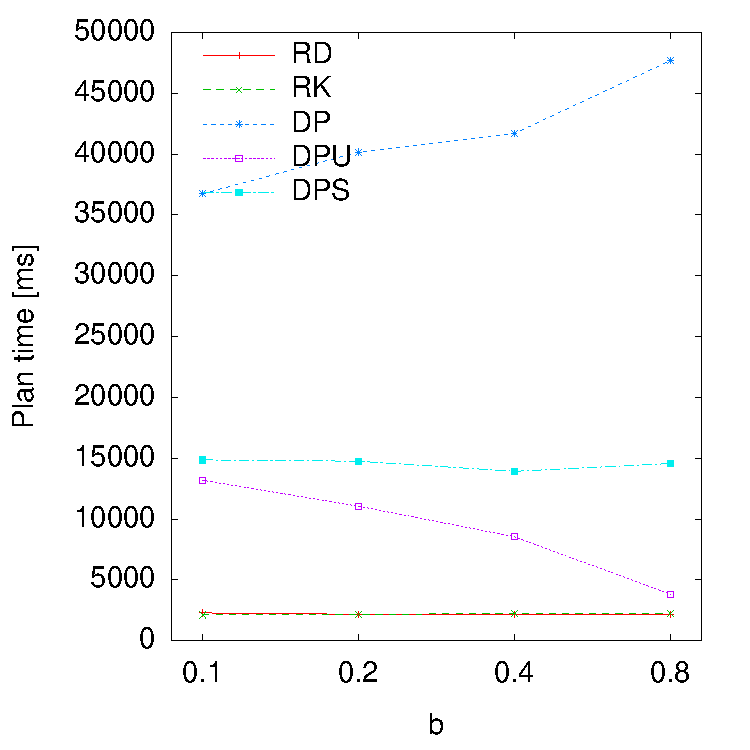
\includegraphics[width=0.49\linewidth]{figs/pareto_plan_b.pdf}
  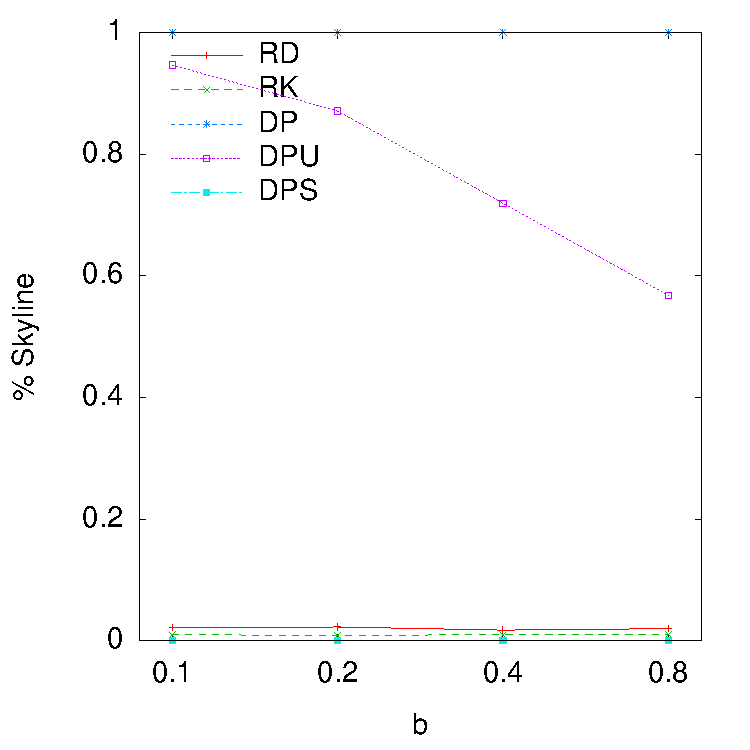
\includegraphics[width=0.49\linewidth]{figs/plans_skyline_by_b.pdf}
  \caption{Effect of sharing benefit on a) planning time and b)
    skyline fractions ($m=2000$).}
  \label{fig:pareto_sharing}
\end{figure}

\textbf{Plan Skyline.} Figs.~\ref{fig:pareto_q2_skyline}a+b show a scatter
plot of cost and cardinality of plans generated by all systems for
query Q2. In these plots a plan dominates all plans that are to its
lower right, i.e. that have higher cost (x-axis) and lower cardinality
(y-axis). Fig.~\ref{fig:pareto_q2_skyline}a shows all plans that were
generated by the different systems. We can immediately see that many
of the plans generated by the RD and RK baselines are dominated by
other plans. Fig.~\ref{fig:pareto_q2_skyline}b shows only the plans
for all systems that are on the skyline. Here, the dominated plans in
the center of the plot no longer appear and only few RD and RK plans
remain.

\begin{figure}[htb]
  \centering
  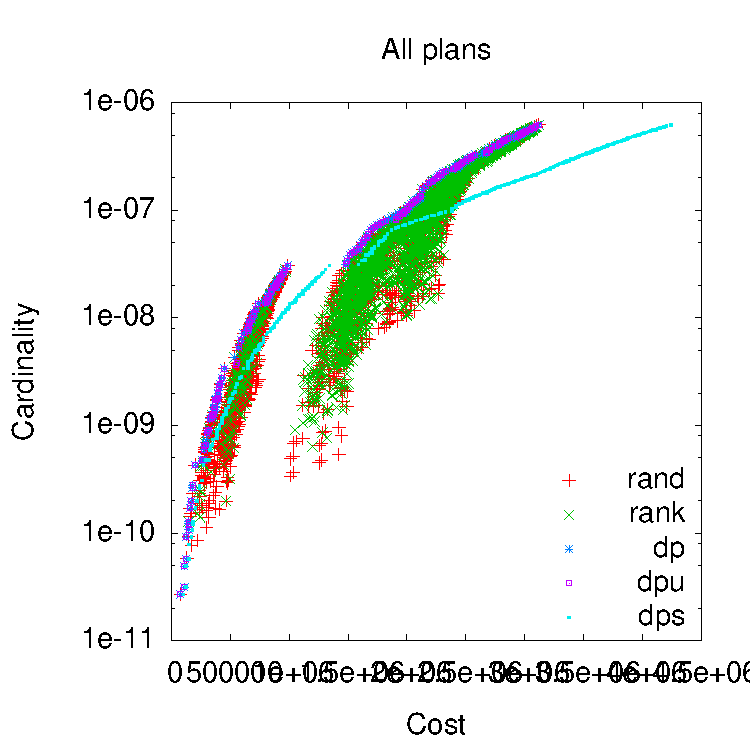
\includegraphics[width=0.49\linewidth]{figs/plans_q2_all.pdf}
  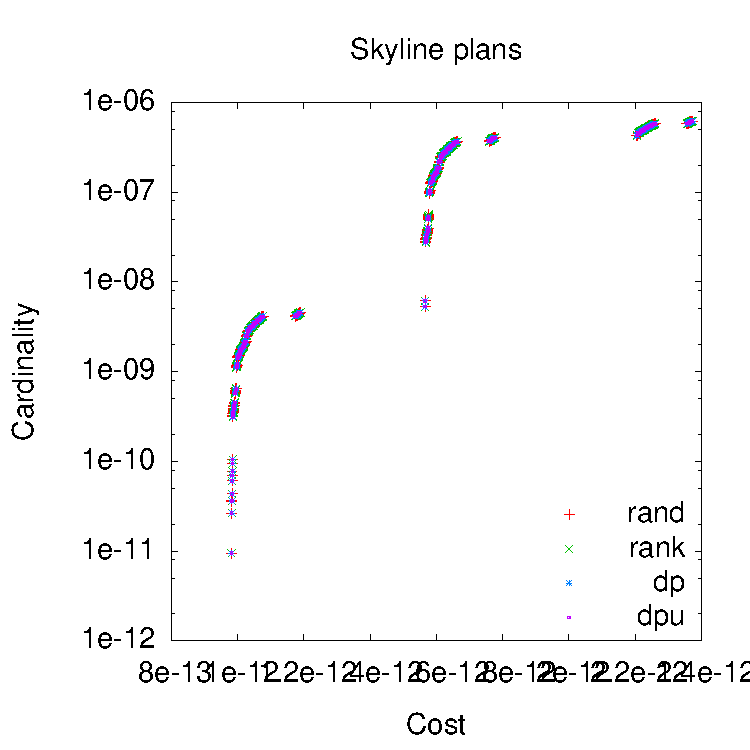
\includegraphics[width=0.49\linewidth]{figs/plans_q2_sky.pdf}
  \caption{Plans for query Q2 on all systems: a) all plans and b)
    skyline plans ($b=0.8,m=2000$).}
  \label{fig:pareto_q2_skyline}
\end{figure}

\textbf{Execution Time.}  Fig.~\ref{fig:exec_q7} shows the execution
times and number of results for 10\% of plans (randomly chosen) for
query Q7 generated by DP. We see that plans that produce less results
in general have shorter execution times. In order to find all 106
query results, the fastest plan takes 17.9 seconds; producing a subset
of 46 results requires only 4.3 seconds.

However, we can also see that some of the plans produce no results at
all. This is due to the fact that the employed cardinality estimation
procedure does not take dependencies between sources into
account. Here, a more sophisticated method for cardinality estimation
would help avoid generting empty plans.

\begin{figure}[htb]
  \centering
  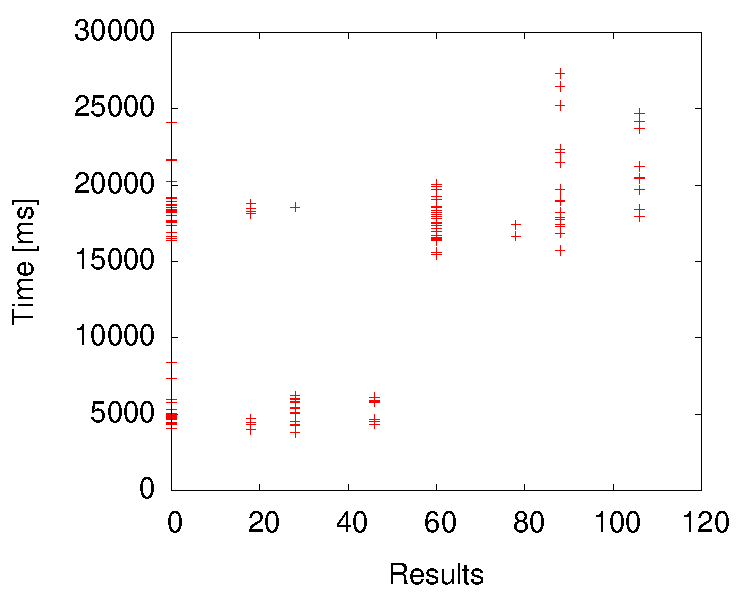
\includegraphics[width=0.8\linewidth]{figs/q7_execution.pdf}
  \caption{Execution times of query plans for query Q7.}
  \label{fig:exec_q7}
\end{figure}
%%% Local Variables: 
%%% mode: latex
%%% TeX-master: "paper"
%%% End: 
